%% contacts_phase1: two-page abstract in ACM format (FNI 421 Mobile Computing, Phase 1).
%%
%% How to build: in Overleaf, upload this file and references.bib to a new project
%% (Overleaf already has the ACM acmart class), or use any TeX Live with pdfLaTeX + BibTeX.
%%
%% Before you submit: replace "Team Member 1..6", "University Name", "City" and "Country"
%% in the author block below with your real details. Keep one \author block per team member
%% and delete the extra ones.
\documentclass[sigconf,nonacm]{acmart}

\usepackage{tikz}
\usetikzlibrary{positioning,arrows.meta}

\begin{document}
% Narrow columns and long code names: let a line get looser instead of letting a word stick out.
\sloppy

\title{contacts\_phase1: A Contact Manager for Android Built with Jetpack Compose, Intents and Room}
\subtitle{FNI 421 Mobile Computing, Phase 1 Project}

\author{Team Member 1}
\affiliation{\institution{University Name}\city{City}\country{Country}}
\author{Team Member 2}
\affiliation{\institution{University Name}\city{City}\country{Country}}
\author{Team Member 3}
\affiliation{\institution{University Name}\city{City}\country{Country}}
\author{Team Member 4}
\affiliation{\institution{University Name}\city{City}\country{Country}}
\author{Team Member 5}
\affiliation{\institution{University Name}\city{City}\country{Country}}
\author{Team Member 6}
\affiliation{\institution{University Name}\city{City}\country{Country}}

\begin{abstract}
This paper describes contacts\_phase1, an Android contact manager that our student team built for
the Phase~1 project of FNI~421 Mobile Computing. The app is written in Kotlin with
Jetpack Compose and Material~3. Contacts and groups are stored in a Room database with full
create, read, update and delete support, while the sort order and the five most recent searches
are kept with Preferences DataStore. Three activities pass a contact's id to each other through
explicit intents, and implicit intents connect a contact to the dialer, messaging, e-mail, maps
and the share sheet; an intent filter also lets other apps share text into a new contact. We
present the architecture, the main features, the problems we found while testing on a real phone
and how we fixed them, and our plans for Phase~2.
\end{abstract}

\ccsdesc[500]{Human-centered computing~Ubiquitous and mobile computing systems and tools}
\ccsdesc[300]{Information systems~Data management systems}

\keywords{Android, Kotlin, Jetpack Compose, Room, DataStore, Intents}

\maketitle

\section{Introduction}
Almost every phone has an address book, which makes it a good subject for a first mobile project:
it needs lists and forms, data that must survive closing the app, and links to other apps such as
the dialer. The Phase~1 rubric asks for feature coverage (Jetpack Compose and Intents), a clean
and responsive UI, clean Kotlin code, and persistence with Room or DataStore. We took the idea of
the open-source ContactList app~\cite{contactlist} and wrote contacts\_phase1 from scratch around
these requirements, following Android's recommended app architecture~\cite{architecture}.
Table~\ref{tab:rubric} maps each rubric item to the parts of the app that cover it.

\begin{table}[t]
  \caption{How the app meets the Phase~1 rubric}
  \label{tab:rubric}
  \small
  \begin{tabular}{@{}p{0.25\columnwidth}p{0.71\columnwidth}@{}}
    \toprule
    Rubric item & Where it is covered \\
    \midrule
    Feature coverage & Every screen in Compose; three activities linked by explicit Intents;
      five implicit Intents and an \texttt{ACTION\_SEND} intent filter \\
    UI/UX & Material~3 with dark mode, adaptive grid for landscape and tablets, errors under each
      field, empty states, recent searches \\
    Code quality & \texttt{val} data classes, lambdas and method references, state hoisting,
      ViewModel and repositories \\
    Persistence & Room with full CRUD, two tables, a foreign key and a migration; DataStore for
      settings \\
    \bottomrule
  \end{tabular}
\end{table}

\section{Design and Architecture}
Figure~\ref{fig:architecture} shows the layers. Each screen is its own activity:
\texttt{MainActivity} shows the list, \texttt{DetailActivity} shows one contact and
\texttt{EditContactActivity} adds or edits one. They start each other with explicit intents that
carry only the contact's id as an extra, and each screen loads the contact itself, so no large
objects travel between activities.

The UI is written entirely in Compose~\cite{compose}. Every screen composable receives one
read-only UI state object and reports user actions through lambdas (state hoisting); it keeps
only small UI details itself, such as keyboard focus. Shared parts, such as the contact photo, are separate composables, and slot parameters
let one member's photo picker and action buttons plug into another member's screen.

\texttt{ContactViewModel} turns the database and the settings into a single \texttt{StateFlow}:
it combines the search results, the groups, the search text, the saved settings and the favorites
filter, and it survives screen rotation. Below it, \texttt{ContactsRepository} wraps the Room
DAO~\cite{room} and \texttt{SettingsRepository} wraps DataStore~\cite{datastore}, so no screen
talks to storage directly.

\begin{figure}[t]
  \centering
  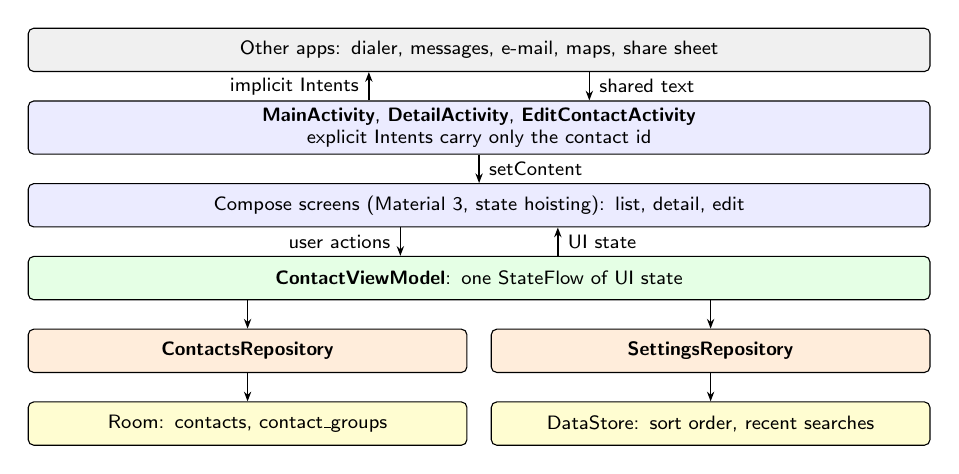
\begin{tikzpicture}[
      font=\sffamily\scriptsize,
      layer/.style={draw, rounded corners=2pt, align=center, inner sep=2.5pt,
        minimum height=5.5mm, text width=#1},
      layer/.default={0.93\columnwidth},
      arrow/.style={-{Stealth[length=3.5pt]}, semithick},
      node distance=3.6mm]
    \node[layer, fill=gray!12] (apps) {Other apps: dialer, messages, e-mail, maps, share sheet};
    \node[layer, fill=blue!8, below=of apps] (acts)
      {\textbf{MainActivity}, \textbf{DetailActivity}, \textbf{EditContactActivity}\\
       explicit Intents carry only the contact id};
    \node[layer, fill=blue!8, below=of acts] (ui) {Compose screens (Material 3, state hoisting): list, detail, edit};
    \node[layer, fill=green!10, below=of ui] (vm) {\textbf{ContactViewModel}: one StateFlow of UI state};
    \node[layer=0.445\columnwidth, fill=orange!14, below=of vm.south west, anchor=north west] (crepo)
      {\textbf{ContactsRepository}};
    \node[layer=0.445\columnwidth, fill=orange!14, below=of vm.south east, anchor=north east] (srepo)
      {\textbf{SettingsRepository}};
    \node[layer=0.445\columnwidth, fill=yellow!18, below=of crepo] (room) {Room: contacts, contact\_groups};
    \node[layer=0.445\columnwidth, fill=yellow!18, below=of srepo] (ds) {DataStore: sort order, recent searches};
    \draw[arrow] ([xshift=-14mm]acts.north) -- node[left] {implicit Intents} ([xshift=-14mm]apps.south);
    \draw[arrow] ([xshift=14mm]apps.south) -- node[right] {shared text} ([xshift=14mm]acts.north);
    \draw[arrow] (acts) -- node[right] {setContent} (ui);
    \draw[arrow] ([xshift=-10mm]ui.south) -- node[left] {user actions} ([xshift=-10mm]vm.north);
    \draw[arrow] ([xshift=10mm]vm.north) -- node[right] {UI state} ([xshift=10mm]ui.south);
    \draw[arrow] (crepo.north |- vm.south) -- (crepo.north);
    \draw[arrow] (srepo.north |- vm.south) -- (srepo.north);
    \draw[arrow] (crepo) -- (room);
    \draw[arrow] (srepo) -- (ds);
  \end{tikzpicture}
  \caption{The layers of contacts\_phase1 and how data moves between them.}
  \Description{A stack of boxes. At the top, other apps exchange implicit intents and shared text
    with the three activities. The activities show Compose screens. The screens send user
    actions to ContactViewModel and receive UI state from it. The ViewModel uses ContactsRepository,
    backed by Room, and SettingsRepository, backed by DataStore.}
  \label{fig:architecture}
\end{figure}

\section{Features}
\begin{itemize}
  \item \textbf{Contacts:} add, view, edit and delete contacts with name, phone, e-mail, city,
    birthday, photo and group. Errors appear under each field, the birthday picker blocks future
    dates, and photos are copied into app storage so they keep working after a restart.
  \item \textbf{Groups:} Family, Work, University and Other, stored in a second table linked by a
    foreign key; deleting a group keeps its contacts.
  \item \textbf{Finding people:} search by name or phone, recent searches under the empty search
    box, an A--Z / Z--A sort that is remembered, and a favorites filter.
  \item \textbf{Other apps~\cite{intents}:} the detail screen can call the contact
    (\texttt{ACTION\_DIAL}), text or e-mail them (\texttt{ACTION\_SENDTO}), show the city on
    a map (\texttt{ACTION\_VIEW} with \texttt{geo:}) and share the contact (\texttt{ACTION\_SEND}
    with a chooser). Text shared from another app opens a new contact with the name, phone and
    e-mail filled in.
  \item \textbf{Look and feel:} Material~3~\cite{material} with dark mode, an adaptive grid that
    shows more columns in landscape and on tablets, and a readable maximum width for forms.
\end{itemize}

\section{Implementation}
All entities are Kotlin data classes whose fields are \texttt{val}, so a contact is never changed
in place: an edit saves a \texttt{copy()} with the new values. Room queries return \texttt{Flow},
so the list and detail screens refresh by themselves after every insert, update or delete, and a
type converter stores birthdays as day numbers. When we added the Other group we raised the
database version to~2 and wrote a migration that inserts the new group, so phones that already
had the app keep all their contacts. DataStore edits are atomic: toggling the sort order reads and
writes inside one \texttt{edit} block, so two quick taps cannot both read the old value.
Coroutines keep database and file work off the main thread.

\section{Testing and Fixes}
We ran the app on a physical Android phone and fixed five problems that testing exposed. (1)~The
search box stayed highlighted after tapping elsewhere; it now lets go of the focus when the user
taps outside it, scrolls, presses the keyboard's Search key or closes the keyboard. (2)~The
favorites filter heart was colored while the filter was off; it is now grey when off and uses the
favorite color when on. (3)~There was no search history; the last five searches now appear under
the empty search box and can be removed. (4)~The three groups did not fit everyone, so we added
Other. (5)~The date picker kept highlighting today after another date was picked; today's ring now
disappears once a date is chosen.

A final code review found more hidden bugs, which we also fixed: a double tap on Save could insert
the same contact twice and a double tap on a contact could open its screen twice, replaced or
deleted photos stayed on the phone, the list briefly showed ``No contacts yet'' at start-up, and an
unreadable settings file would have crashed the app.

\section{Teamwork}
We split the work into six areas: project setup and activities, the Room database, the
repositories and ViewModel, the theme and list screen, the detail and edit screens, and the
intents and photo picker; each member owned one or more of them. Everyone worked on a personal
branch on GitHub and opened pull requests, committing one file per commit with Conventional Commit
messages, so each person's work is visible in the history. Pull requests were merged in dependency
order, from the project setup and database to the activities, so the app compiled after every merge.

\section{Conclusion and Future Work}
contacts\_phase1 covers every Phase~1 requirement with a small, layered code base that each member
can explain. Our main lessons were that a real phone shows problems an emulator hides, such as
keyboard and focus behaviour; that state hoisting and slot parameters let several people build
one app without blocking each other; and that a database change needs a migration before users
have data, not after. For Phase~2 we plan to add unit tests with JUnit and Mockito, search by e-mail and city
and ignore spaces in phone numbers, offer undo after a delete, ask before discarding unsaved edits,
compress photos, and translate the app into Arabic.

\bibliographystyle{ACM-Reference-Format}
\bibliography{references}

\end{document}
